\documentclass[border=6pt]{standalone}
% Shared preamble of every figure (included by each fig*.tex)
\usepackage{fontspec}
\setmainfont{DejaVu Sans}
\setmonofont{DejaVu Sans Mono}
\usepackage{amsmath,amssymb}
\usepackage{tikz}
\usetikzlibrary{positioning,arrows.meta,fit,calc,decorations.pathreplacing,shapes.geometric,backgrounds}
\definecolor{cdata}{HTML}{4C78A8}
\definecolor{cmodel}{HTML}{F58518}
\definecolor{chead}{HTML}{54A24B}
\definecolor{cgold}{HTML}{E45756}
\definecolor{cgrey}{HTML}{9D9D9D}
\definecolor{cfull}{HTML}{B279A2}
\tikzset{
  box/.style={draw, rounded corners=2pt, align=center, inner sep=4pt, font=\small, minimum height=8mm},
  data/.style={box, fill=cdata!15, draw=cdata!80!black},
  model/.style={box, fill=cmodel!18, draw=cmodel!80!black},
  head/.style={box, fill=chead!18, draw=chead!70!black},
  note/.style={font=\footnotesize, align=center, text=black!70},
  arr/.style={-{Stealth[length=2.2mm]}, thick, black!70},
}

\tikzset{blk/.style={draw, align=left, font=\footnotesize\ttfamily, inner sep=3pt, text width=105mm, anchor=north west}}
\begin{document}
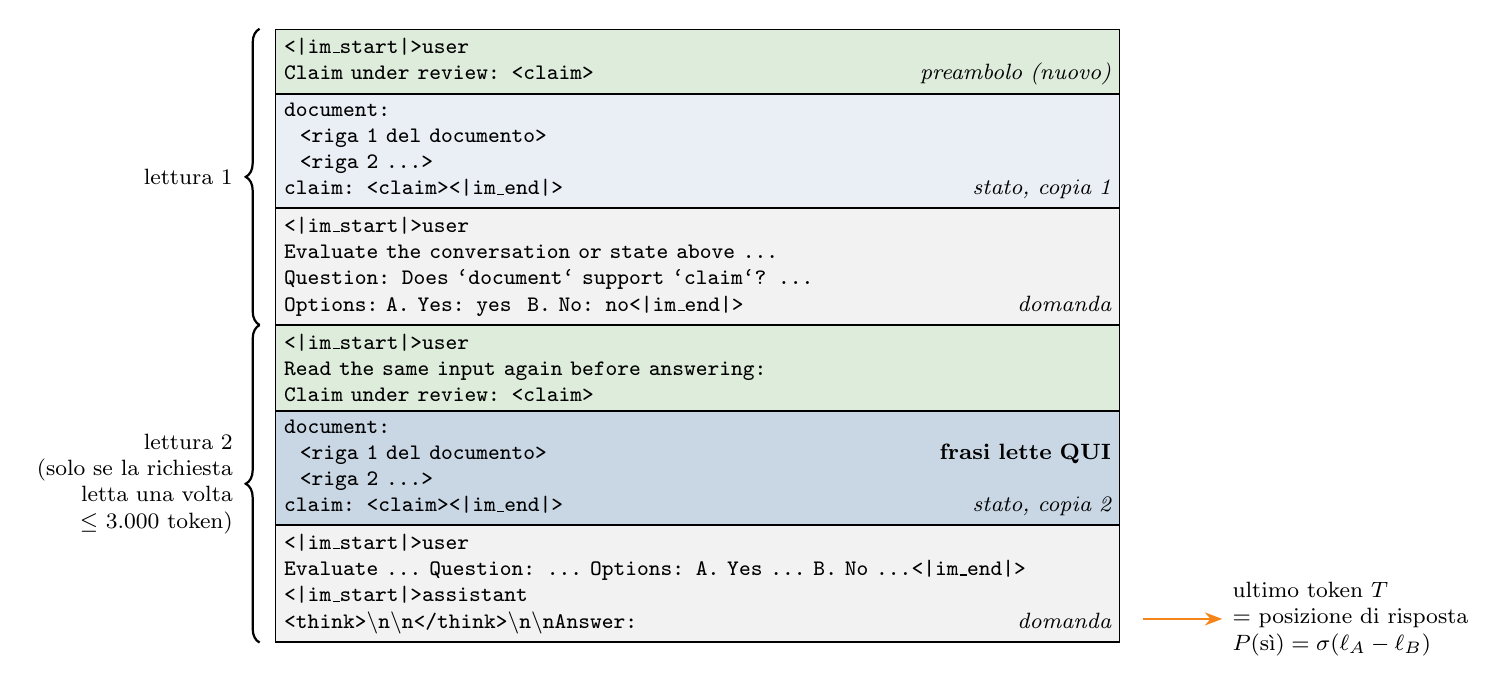
\begin{tikzpicture}
\node[blk, fill=chead!20] (p1) at (0,0) {<|im\_start|>user\\Claim under review: <claim>\hfill\normalfont\itshape preambolo (nuovo)};
\node[blk, fill=cdata!12, ] (s1) at (p1.south west) {document:\\\ \ <riga 1 del documento>\\\ \ <riga 2 \dots>\\claim: <claim><|im\_end|>\hfill\normalfont\itshape stato, copia 1};
\node[blk, fill=black!5, ] (q1) at (s1.south west) {<|im\_start|>user\\Evaluate the conversation or state above \dots\\Question: Does `document` support `claim`? \dots\\Options:\ A. Yes: yes\ \ B. No: no<|im\_end|>\hfill\normalfont\itshape domanda};
\node[blk, fill=chead!20, ] (p2) at (q1.south west) {<|im\_start|>user\\Read the same input again before answering:\\Claim under review: <claim>};
\node[blk, fill=cdata!30, ] (s2) at (p2.south west) {document:\\\ \ <riga 1 del documento>\hfill\textnormal{\textbf{frasi lette QUI}}\\\ \ <riga 2 \dots>\\claim: <claim><|im\_end|>\hfill\normalfont\itshape stato, copia 2};
\node[blk, fill=black!5, ] (q2) at (s2.south west) {<|im\_start|>user\\Evaluate \dots\ Question: \dots\ Options: A. Yes \dots\ B. No \dots<|im\_end|>\\<|im\_start|>assistant\\<think>\textbackslash n\textbackslash n</think>\textbackslash n\textbackslash n\textbf{Answer:}\hfill\normalfont\itshape domanda};
\draw[decorate, decoration={brace, amplitude=5pt, mirror}, thick] ($(p1.north west)+(-2mm,0)$) -- node[left=6pt, font=\footnotesize, align=right] {lettura 1} ($(q1.south west)+(-2mm,0)$);
\draw[decorate, decoration={brace, amplitude=5pt, mirror}, thick] ($(p2.north west)+(-2mm,0)$) -- node[left=6pt, font=\footnotesize, align=right] {lettura 2\\(solo se la richiesta\\letta una volta\\$\le$ 3.000 token)} ($(q2.south west)+(-2mm,0)$);
\draw[arr, cmodel] ($(q2.south east)+(3mm,3mm)$) -- ++(10mm,0) node[right, font=\footnotesize, align=left, text=black] {ultimo token $T$\\= posizione di risposta\\$P(\text{sì}) = \sigma(\ell_A - \ell_B)$};
\end{tikzpicture}
\end{document}
